\documentclass[leqno]{beamer}
\usetheme{CambridgeUS}    %  other good options:   Singapore, Warsaw, Plain, CambridgeUS, Berlin

%\mode<presentation> {
 % \setbeamertemplate{background canvas}[vertical shading][bottom=white!10,top=white!10]
 %\setbeamertemplate{navigation symbols}{}
 
  %\usefonttheme[onlysmall, nonav]{structurebold}
%}
\usepackage{graphics,multicol,url}
\usepackage{colortbl}
% \usepackage{biblatex}
% \bibliography{JetBib.bib}
\usepackage{amsfonts, amsmath, amssymb, eucal, enumerate,calc,latexsym,amsfonts}
\usepackage{amsmath,amsthm, amssymb, latexsym}
\usepackage{enumerate}
\usepackage{tikz}
\usetikzlibrary{shadings}
\usepackage{gensymb}

\usepackage{amssymb, amsthm, amsmath, amsfonts}
\usepackage{cancel, enumerate, url, mathrsfs}
% \input{dvipsnam.def}
% \usepackage{graphicx}
% \DeclareGraphicsRule{.tif}{png}{.png}{`convert #1 `dirname #1`/`basename #1 .tif`.png}
% \graphicspath{{./figures/}}
 \setbeamertemplate{navigation symbols}{}    % removes the panel with navigation symbols from the lower right corner
% Shows "invisible text"
%\setbeamercovered{still covered={\opaqueness<1->{5}}}

%\setbeameroption{show notes}
%\setbeameroption{show notes on side=left}


\newtheorem{thm}{Theorem}
\newtheorem{cor}[thm]{Corollary}
\newtheorem{lem}[thm]{Lemma}
\newtheorem{prop}[thm]{Proposition}
\theoremstyle{definition}
\newtheorem{defn}[thm]{Definition}
\theoremstyle{remark}
\newtheorem{rem}[thm]{Remark}
%\numberwithin{equation}{section}



\newcommand{\vp}{\varphi}
\newcommand{\re}{\mathbb{R}}
\newcommand{\na}{\mathbb N}
\newcommand{\ra}{\mathbb Q}
\newcommand{\bfx}{\bf x}
\newcommand{\ds}{\displaystyle}
\newcommand{\dint}{\displaystyle\int}
\newcommand{\al}{\alpha}
\definecolor{DarkBlue}{rgb}{0.1,0.1,0.5}
\definecolor{Red}{rgb}{0.9,0.0,0.1}
\newcommand{\brown}[1]{{\color{brown} #1}}
\newcommand{\red}[1]{{\color{red} #1}}
\newcommand{\blue}[1]{{\color{blue} #1}}


\title[Math 107-Lecture 8]{Calculus I - Lecture 8\\Friday, September 8, 2017}
\author[A. Larios]{Dr. Adam Larios}
\institute[UNL]{University of Nebraska-Lincoln}
\date{September 8, 2017}

\begin{document}

\frame{\titlepage}
%%%%%%%%%%%%%%%%%%%%%%%%%%%%%%%%%%%%%%%%%%%%%%%%%%%%%%%%%%%


\begin{frame}
\frametitle{Announcements}

\begin{itemize}
\item Today: differentiability and the second order derivative (sections 2.5 and 2.6).
\end{itemize}
\end{frame}



%%%%%%%%%%%%%%%%%%%%%%%%%%%%%%%%%%%%%%%%%%%%%%%%%%%%%%%%%%%


\frame{\frametitle{Differentiability}

{\color{blue}Definition.}  A function $f(x)$ is differentiable at $x$ if 
\[
\lim_{h\to 0} \frac{f(x+h)-f(x)}{h}
\]
exists. If $f(x)$ is differentiable at $x=a$ then its graph has a {\color{red}non-vertical} tangent line at $x=a$. {\color{red}What can go wrong?} 

\begin{multicols}{3}
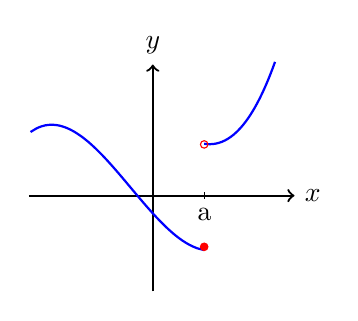
\begin{tikzpicture}[scale=0.45]

    \draw[->,thick] (-3.5,0) -- (4,0) node[right] {$x$};
    \draw[->,thick] (0,-2.7) -- (0,3.7) node[above] {$y$};
	\draw (1.45,0.1) -- (1.45, -0.1) node[below] {a};

\draw[-,color=blue,smooth,domain=-3.45:1.45,thick] plot(\x,{\x*(\x)*(\x)*0.08+(\x)*(\x)*0.15-1.1*\x-0.5});
\draw[-,color=blue,smooth,domain=1.45:3.45,thick] plot(\x,{\x*(\x)*(\x)*0.08+(\x)*(\x)*0.15-1.1*\x+2.5});
\draw[color=red] (1.45,-1.445) circle[radius=3pt];
\fill[color=red] (1.45,-1.445) circle[radius=3pt];
\draw[color=red] (1.45,1.445) circle[radius=3pt];
\end{tikzpicture}


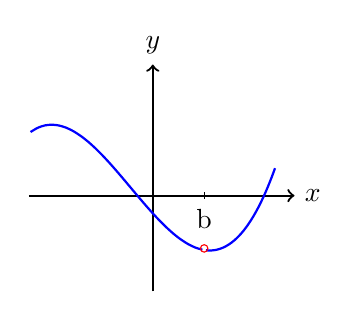
\begin{tikzpicture}[scale=0.45]

    \draw[->,thick] (-3.5,0) -- (4,0) node[right] {$x$};
    \draw[->,thick] (0,-2.7) -- (0,3.7) node[above] {$y$};
	\draw (1.45,0.1) -- (1.45, -0.1) node[below] {b};

\draw[-,color=blue,smooth,domain=-3.45:1.4,thick] plot(\x,{\x*(\x)*(\x)*0.08+(\x)*(\x)*0.15-1.1*\x-0.5});
\draw[-,color=blue,smooth,domain=1.5:3.45,thick] plot(\x,{\x*(\x)*(\x)*0.08+(\x)*(\x)*0.15-1.1*\x-0.5});
\draw[color=red] (1.45,-1.49) circle[radius=3pt];
%\fill[color=red] (1.45,-1.445) circle[radius=3pt];
%\draw[color=red] (1.45,1.445) circle[radius=3pt];
\end{tikzpicture}

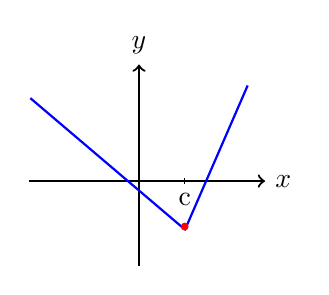
\begin{tikzpicture}[scale=0.4]

    \draw[->,thick] (-3.5,0) -- (4,0) node[right] {$x$};
    \draw[->,thick] (0,-2.7) -- (0,3.7) node[above] {$y$};
	\draw (1.45,0.1) -- (1.45, -0.1) node[below] {c};

\draw[-,color=blue,smooth,domain=-3.45:1.45,thick] plot(\x,{(-.85)*(\x)-0.3});
\draw[-,color=blue,smooth,domain=1.45:3.45,thick] plot(\x,{\x*(2.3)-4.9});
\draw[color=red] (1.45,-1.445) circle[radius=3pt];
\fill[color=red] (1.45,-1.445) circle[radius=3pt];
\end{tikzpicture}

\end{multicols}

\hspace*{1in} (a), (b) discontinuities; \hspace*{1in} (c) ``corner"}


%%%%%%%%%%%%%%%%%%%%%%%%%%%%%%%%%%%%%%%%%%%%%%%%%%%%%%%%%%%

\frame{\frametitle{What can go wrong?(cont.)} 

\begin{multicols}{2}

\begin{tikzpicture}[scale=0.5]

    \draw[->,thick] (-3,0) -- (4,0) node[right] {$x$};
    \draw[->,thick] (0,-2.7) -- (0,3.7) node[above] {$y$};
	\draw (-2,0.1) -- (-2, -0.1) node[below] {d};
	
	\draw[-,color=blue,smooth,domain=-4:-1,thick] plot(\x,{sqrt(4-(\x+3)*(\x+3))});
\draw[-,color=blue,smooth,domain=-1:2.3,thick] plot(\x,{sqrt(4-(\x-1)*(\x-1))});


\end{tikzpicture}


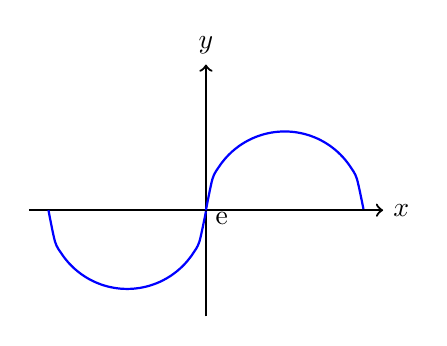
\begin{tikzpicture}[scale=0.5]

    \draw[->,thick] (-4.5,0) -- (4.5,0) node[right] {$x$};
    \draw[->,thick] (0,-2.7) -- (0,3.7) node[above] {$y$};
	\draw (0,0.2) -- (0, -0.2) node[right] {e};

\draw[-,color=blue,smooth,domain=0:4,thick] plot(\x,{sqrt(4-(\x-2)*(\x-2))});
\draw[-,color=blue,smooth,domain=-4:0,thick] plot(\x,{(-1)*sqrt(4-(\x+2)*(\x+2))});


\end{tikzpicture}

\end{multicols}

(d) = cusp; \hspace*{2in}(e)=vertical asymptote.
}



%%%%%%%%%%%%%%%%%%%%%%%%%%%%%%%%%%%%%%%%%%%%%%%%%%%%%%%%%%%
\frame{\frametitle{More non-differentiability}
{\color{blue}Example.} Is $f(x)=x+|x|$ differentiable at $x=0$? 
\pause
\[
f(x)=\begin{cases}
2x, \quad x\geq 0\\
0,\quad x<0.
\end{cases}
\]
Then everything is well everywhere, except at $x=0$.
\[
\lim_{h\to 0+} \frac{f(h)-f(0)}{h}=2
\]
\pause
While
\[
\lim_{h\to 0-} \frac{f(h)-f(0)}{h}=0
\]
Since the side limits do not agree, the limit does not exist. Hence, {\color{red}$f$ is not differentiable at $x=0$}.
}



%%%%%%%%%%%%%%%%%%%%%%%%%%%%%%%%%%%%%%%%%%%%%%%%%%%%%%%%%%%

\frame{\frametitle{Clicker question \#1}
Which of the functions below are differentiable?
\begin{enumerate}[(A)]
\item $|x|^2$
\item $|x|^2-2|x|$
\item $|x+5|$
\item $\sqrt{(x+2)^2}$
\item $3-|x|$
\end{enumerate}
}


%%%%%%%%%%%%%%%%%%%%%%%%%%%%%%%%%%%%%%%%%%%%%%%%%%%%%%%%%%%

\frame{\frametitle{Differentiable $\implies$ continuous}
{\color{blue}Theorem.}  If $f(x)$ is differentiable at $x=a$ then $f$ is continuous at $x=a$

\vspace*{.3in}

{\color{red} The converse is not true! } There are continuous functions which are not differentiable (see graphs (c), (d), (e) above).
}

%%%%%%%%%%%%%%%%%%%%%%%%%%%%%%%%%%%%%%%%%%%%%%%%%%%%%%%%%%%

\frame{\frametitle{Second order derivatives}
The derivative of the derivative function is {\color{blue}the second order derivative}:
\[
f''(x)=\lim_{h\to 0}\frac{f'(x+h)-f'(x)}{h}
\]
provided the limit exists.

{\color{blue}Example.} Find $f''(x)$ for $f(x)=2x^2+3x.$
\pause

Last time we showed that $f'(x)=4x+3$, so we compute 
\begin{align*}
f''(x)&=\lim_{h\to 0}\frac{f'(x+h)-f'(x)}{h}\\
&=\lim_{h\to 0}\frac{4(x+h)+3-4x-3}{h}\\
&=4.
\end{align*}
}

%%%%%%%%%%%%%%%%%%%%%%%%%%%%%%%%%%%%%%%%%%%%%%%%%%%%%%%%%%%

\frame{\frametitle{Notation}
If $y=f(x)$, then
\[
f''(x)=y''=\frac{d^2y}{dx^2}=\frac{d^2f}{dx^2}=\frac{d}{dx}\left[\frac{dy}{dx}\right]=\frac{d}{dx}[f'(x)] ...
\]

}



%%%%%%%%%%%%%%%%%%%%%%%%%%%%%%%%%%%%%%%%%%%%%%%%%%%%%%%%%%%

\frame{\frametitle{Concavity and convexity}
For $f$ a function
\begin{itemize}
\item the sign of $f$ gives the monotonicity (increasing vs. decreasing)
\item the sign of $f''$ gives the concavity/convexity as follows
\begin{enumerate}
\item If $(f')'>0$ then the slope of $f'$ is increasing; hence, the shape is concave up/convex (the graph ``holds water'')
\item If $(f')'<0$ then the slope of $f'$ is decreasing; hence, the shape is concave down (the graph `` does not hold water'')
\end{enumerate}
\end{itemize}


\begin{multicols}{2}

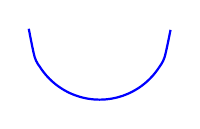
\begin{tikzpicture}[scale=0.45]
\draw[-,color=blue,smooth,domain=-1:3,thick] plot(\x,{-sqrt(4-(\x-1)*(\x-1))});
\end{tikzpicture}

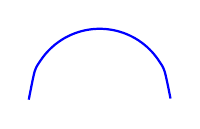
\begin{tikzpicture}[scale=0.45]
\draw[-,color=blue,smooth,domain=0:4,thick] plot(\x,{sqrt(4-(\x-2)*(\x-2))});
\end{tikzpicture}
\end{multicols}
Concave up (convex) \hspace*{0.8in}
Concave down 

}


%%%%%%%%%%%%%%%%%%%%%%%%%%%%%%%%%%%%%%%%%%%%%%%%%%%%%%%%%%%

\frame{\frametitle{Analyzing concavity}
For $f(x)=x^3+2x$ we show that $f'(x)=3x^2+2$ and $f''(x)=6x.$
Hence
\begin{itemize}
\item $f$ is increasing everywhere as $f'(x)=3x^2+2>0$ for all $x\in \re$
\item $f$ is concave up whenever $f''(x)=6x>0$ (hence for $x>0$) and it is concave down whenever $f''(x)=6x<0$ (for $x<0$).
\end{itemize}

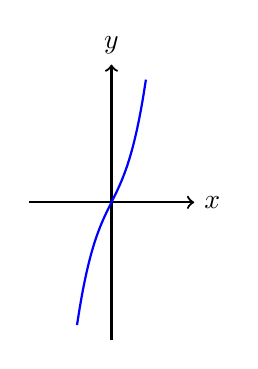
\begin{tikzpicture}[scale=0.35]

    \draw[->,thick] (-3,0) -- (3,0) node[right] {$x$};
    \draw[->,thick] (0,-5) -- (0,5) node[above] {$y$};

\draw[-,color=blue,smooth,domain=-1.25:1.25,thick] plot(\x,{\x^3+2*\x});


\end{tikzpicture}

}


%%%%%%%%%%%%%%%%%%%%%%%%%%%%%%%%%%%%%%%%%%%%%%%%%%%%%%%%%%%

\frame{\frametitle{Clicker question \#2}
If the derivative of $f$ is $f'(x)=2x^2+4x$, on which interval is the function $f$ concave up?
\begin{enumerate}[(A)]
\item $(-\infty, \infty)$
\item $(-\infty, 0)$
\item $(0, \infty)$
\item $(-1, \infty)$
\item $(2, \infty)$
\end{enumerate}
}


%%%%%%%%%%%%%%%%%%%%%%%%%%%%%%%%%%%%%%%%%%%%%%%%%%%%%%%%%%%
\frame{\frametitle{Acceleration}
Assume that $y=s(t)$ gives the position at time $t$ of an object. Then
\begin{itemize}
\item $v(t)=\ds\frac{dy}{dt}=s'(t)$ is the velocity at time $t$ (units of length/time)
\item $a(t)=\ds\frac{d^2y}{dt^2}=v'(t)=s''(t)$ provides the acceleration at time $t$ (units of length/time$^2$).  
\end{itemize}

}


%%%%%%%%%%%%%%%%%%%%%%%%%%%%%%%%%%%%%%%%%%%%%%%%%%%%%%%%%%%

\frame{\frametitle{Position, velocity, acceleration}
Suppose that an object's {\bf velocity} is given by the graph:

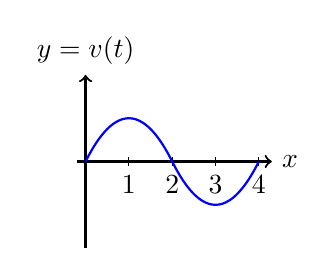
\begin{tikzpicture}[scale=0.55]

    \draw[->,thick] (-0.2,0) -- (4.3,0) node[right] {$x$};
    \draw[->,thick] (0,-2) -- (0,2) node[above] {$y=v(t)$};
\foreach \x in {1,2,3,4} \draw (\x,0.1) -- (\x, -0.1) node[below] {\x};

\draw[-,color=blue,smooth,domain=0:2,thick] plot(\x,{1-(\x-1)^2)});
\draw[-,color=blue,smooth,domain=2:4,thick] plot(\x,{(\x-3)^2-1});
\end{tikzpicture}
\begin{itemize}
\item On what intervals is the acceleration positive?
\item On what intervals is the object's position increasing?
\item Where is the function $s(t)$ increasing/decreasing, concave up/concave down?
\item Suppose that $s(0)=1$. Sketch a possible graph for $s$.  
\end{itemize}
}


%%%%%%%%%%%%%%%%%%%%%%%%%%%%%%%%%%%%%%%%%%%%%%%%%%%%%%%%%%%





\begin{frame}

\frametitle{Wrapping up}
For next time
\begin{itemize}
\item Work on the suggested problems from sections 2.5 and 2.6  (from syllabus and webwork).
\item Read sections 3.1 and 3.2 (derivatives of polynomials and exponentials).
\end{itemize}

\end{frame}

\end{document}
